\documentclass[11pt]{scrartcl}

\usepackage[sexy]{evan}
\usepackage{pgfplots}
\pgfplotsset{compat=1.15}
\usepackage{mathrsfs}
\usetikzlibrary{arrows}
\usepackage{graphics}
\usepackage{tikz}
\usepackage{ amssymb }
\usepackage[dvipsnames]{xcolor}
\usepackage[utf8]{inputenc}
\usepackage{longtable}
\usepackage{ragged2e}
\usepackage{listings}
\definecolor{red1}{RGB}{255, 153, 153}
\definecolor{green1}{RGB}{204, 255, 204}
\definecolor{blue1}{RGB}{204, 255, 255}
\definecolor{yellow1}{RGB}{255, 247, 160}

\definecolor{red2}{RGB}{255, 102, 102}
\definecolor{green2}{RGB}{108, 255, 108}
\definecolor{blue2}{RGB}{94, 204, 255}
\definecolor{yellow2}{RGB}{255, 250, 104}

\definecolor{red2.5}{RGB}{255,76,76}
\definecolor{green2.5}{RGB}{54, 247, 54}
\definecolor{blue2.5}{RGB}{51, 189, 255}
\definecolor{yellow2.5}{RGB}{255, 242, 52}


\definecolor{red3}{RGB}{255, 51, 51}
\definecolor{green3}{RGB}{0, 240, 0}
\definecolor{blue3}{RGB}{9, 175, 255}
\definecolor{yellow3}{RGB}{255, 234, 0}

\definecolor{red3.5}{RGB}{229, 25, 25}
\definecolor{green3.5}{RGB}{0, 194, 0}
\definecolor{blue3.5}{RGB}{4, 143, 209}
\definecolor{yellow3.5}{RGB}{255,220,0}

\definecolor{red4}{RGB}{204, 0, 0}
\definecolor{green4}{RGB}{0, 149, 0}
\definecolor{blue4}{RGB}{0, 111, 164}
\definecolor{yellow4}{RGB}{255, 206, 0}


\definecolor{noseve}{RGB}{242,242,242}

\newcommand{\camod}[1]{\frac{\ZZ}{#1 \ZZ}}
\newcommand{\modm}[1]{\text{ mod } #1}
\newcommand{\campm}[1]{\frac{\ZZ}{m\ZZ}}

\usepackage{epigraph}
\renewcommand{\epigraphsize}{\scriptsize}
\renewcommand{\epigraphwidth}{60ex}


\definecolor{dcol0}{HTML}{C8E6C9}
\definecolor{dcol1}{HTML}{D4E9B3}
\definecolor{dcol2}{HTML}{E5ED9A}
\definecolor{dcol3}{HTML}{FFF59D}
\definecolor{dcol4}{HTML}{FFE082}
\definecolor{dcol5}{HTML}{FFCC80}
\definecolor{dcol6}{HTML}{FFAB91}
\definecolor{dcol7}{HTML}{F49890}
\definecolor{dcol8}{HTML}{E57373}
\definecolor{dcol9}{HTML}{D32F2F}

\makeatletter
\newcommand{\getcolorname}[1]{dcol#1}
\makeatother

\newcommand{\dif}[1]{%
    \edef\colorindex{\number\fpeval{floor(#1)}}%
    \edef\fulltext{#1}%
    \colorbox{\getcolorname{\colorindex}}{%
        \ifnum\colorindex>8
            \textbf{\textcolor{white}{\,\fulltext\,}}%
        \else
            \textbf{\textcolor{black}{\,\fulltext\,}}%
        \fi
    }%
}
% Variable para dificultad (inicial 0)
\newcommand{\thmdifficulty}{0}

% Comando para asignar dificultad antes del problema
\newcommand{\problemdiff}[1]{\renewcommand{\thmdifficulty}{#1}}

% Estilo del problema que incluye dificultad antes del título
\declaretheoremstyle[
    headfont=\color{blue!40!black}\normalfont\bfseries,
    headformat={%
      \dif{\thmdifficulty}\quad \NAME~\NUMBER\ifx\relax\EMPTY\relax\else\ \NOTE\fi
    },
    postheadspace=1em,
    spaceabove=8pt,
    spacebelow=8pt,
    bodyfont=\normalfont
]{problemstyle}

    \declaretheorem[style=problemstyle,name=Problema,sibling=theorem]{problema}
    \declaretheorem[style=problemstyle,name=Problema,numbered=no]{problema*}


\title {10.- Bootstrap (Act 2)}
\subtitle{Programación WEB I \\ Centro de Enseñanza Tecnica Industrial}
\date{16 de Octubre de 2025}
\author{Emmanuel Buenrostro 22300891 7F1}


\begin{document}

\maketitle


\begin{center}
   
\includegraphics[scale=0.15]{../cetilogo.jpg} 
\end{center}
\newpage
\tableofcontents


\section{Resumen}
Bootstrap es un framework de desarrollo web, el cual consta de distintos scripts que le dan al programador distintas opciones, como una cuadricula o distintos componentes para poder programar una interfaz de usuario responsiva especialmente para celular.
\section{Desarrollo}

\subsection{¿Qué es Bootstrap?}

Bootstrap es un framework de desarrollo web gratuito y de codigo abierto.  \\
Esta diseñado para que sera más facil el proceso de desarrollar paginas web responsivas y sobretodo orientadas para moviles. 

Consta  de scripts basados en HTML, CSS y JS para ofrecer diversas funciones y componentes de manera mas sencilla. \\

Además cuenta con una cuadricula de filas y coolumnas, las cuales puede definir breakpoints en base al tamaño de la pantalla, lo cual puede hacer que  
en pantallas de celular se muestre el contenido de una forma mas clara al usuario.  \\


Cuenta además con distintos componentes como:
\begin{itemize}
    \item Botones o formularios
    \item Navbars
    \item Cards
    \item Carruseles
    \item Ventanas emergentes
    \item Alertas
    \item Barra de progreso
\end{itemize}



Además de eso cuenta con clases para css, las cuales sirven para poder definir propiedades del estilo css de un componente solo poniendo ciertas etiquetas mas chicas en su class, haicendolo más facil de 
identificar.

También cuenta con distintos codigos en JS que le pueden agregar funcionalidad a los componentes como desplegar.


\subsection{Ventajas}

Sus ventajas son que al tener varios componentes y estilo predefinidos se pueden crear 
interfaces de usuario bastante mas rapido.  \\

Tambien que es la manera más facil de crear un sitio web responsive, tener una mejor consistencia visual ya que todos los elementos tengan el mismo estilo. \\

Además de contar con una curva de aprendizaje relativamente baja y tiene bastante documentación.


\subsection{Desventajas}

Tiene bastantes funciones 

\subsection{Ejemplo Tienda de Ropa}

Un ejemplo es esta tienda de ropa la cual tiene sus productos en \textit{Card}, y las cuales estan acomodadas de una forma que no se sale de la pantalla, aunque esta se haga más chica. 

\begin{center}
    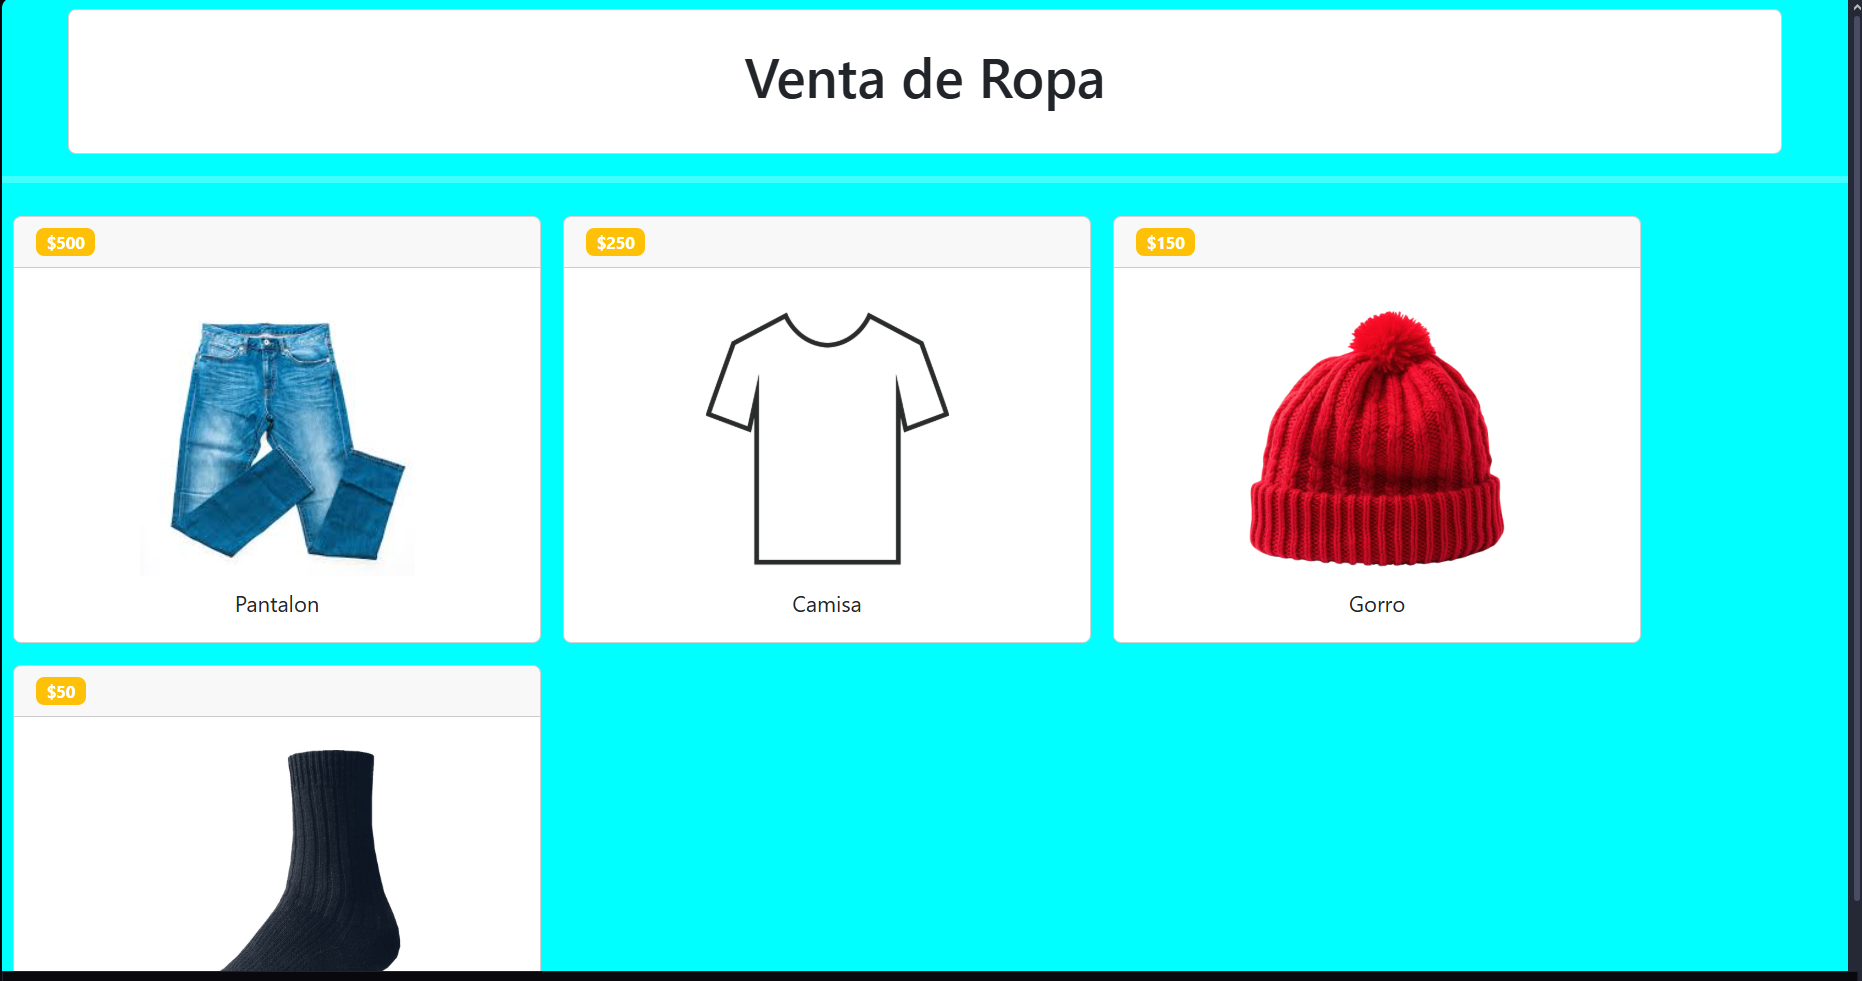
\includegraphics[scale=0.4]{img1.png}
\end{center}
\begin{center}
    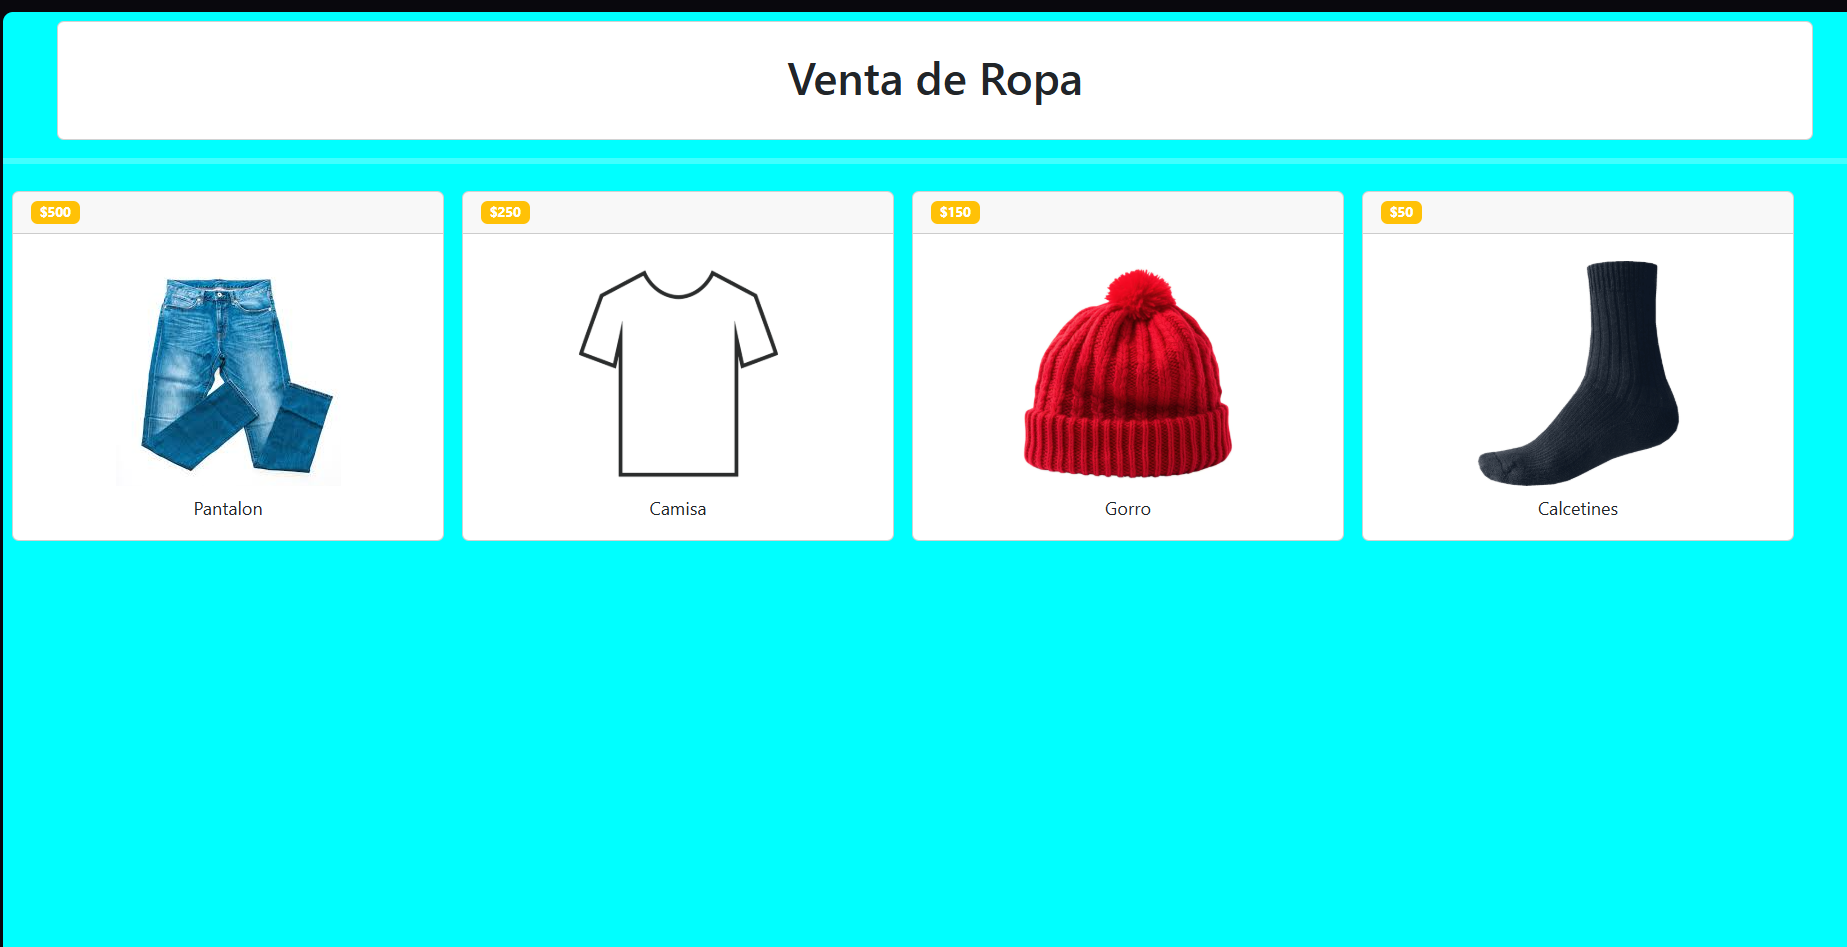
\includegraphics[scale=0.4]{img2.png}
\end{center}
\begin{center}
    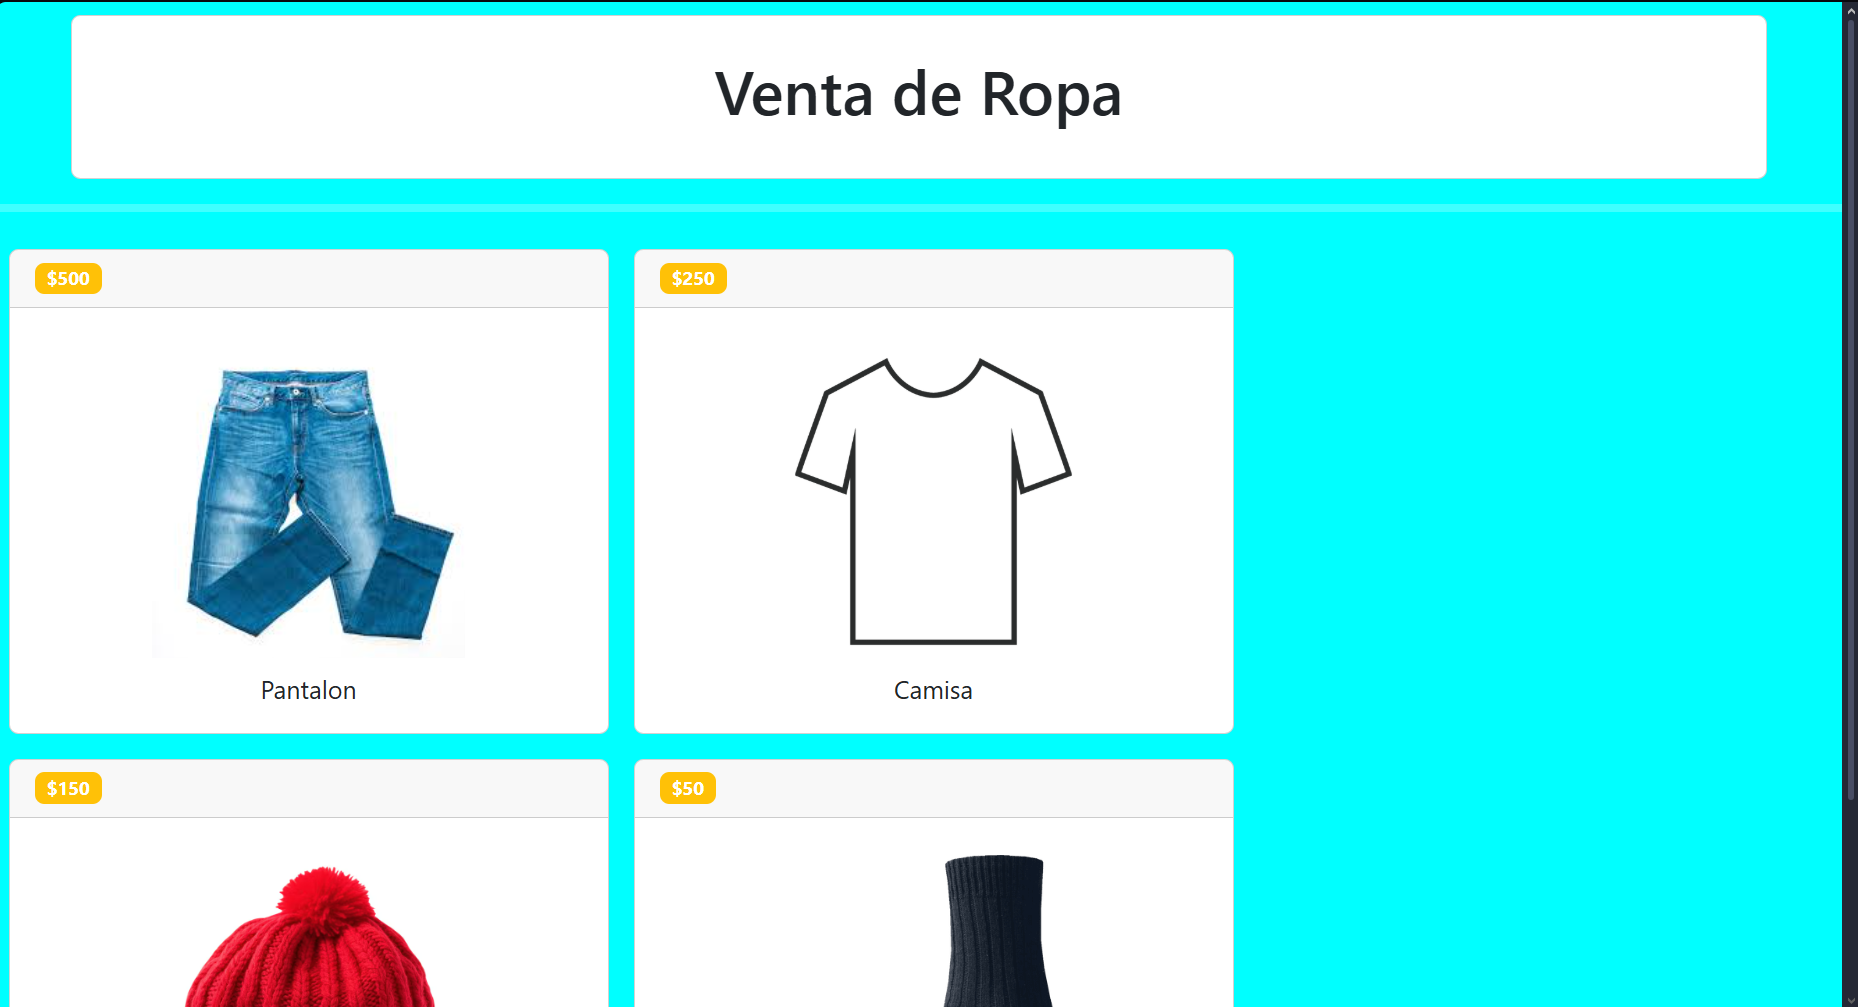
\includegraphics[scale=0.4]{img3.png}
\end{center}



\section{Conclusión}
Bootstrap es una herramienta bastante util para facilitar al programador el diseñar interfaces de usuario para distintos dispositivos/navegadores, además de tener distintas herramientas integradas.

    \section{Bibliografía}

\begin{itemize}
    \item  A, D.,  A, D. (2023, 11 enero). ¿Qué es Bootstrap? - una guía para principiantes. Tutoriales Hostinger. \url{https://www.hostinger.com/mx/tutoriales/que-es-bootstrap} 
    \item Arsys. (s. f.). Guía completa sobre Bootstrap. \url{https://www.arsys.es/blog/guia-completa-sobre-bootstrap}
    \item Calvo, L. (2024, 23 febrero). ¿Qué es Bootstrap? Guía para diseñadores y desarrolladores web. GoDaddy Resources - Spain. \url{https://www.godaddy.com/resources/es/crearweb/que-es-bootstrap}
    \item Carolina. (2025, 18 septiembre). Bootstrap: ¿qué es, para qué sirve y cómo instalarlo? Pingback. \url{https://pingback.com/es/resources/bootstrap} 
    \item The Coder Cave, Programación y Tecnología. (2021, 30 julio). Aprende Bootstrap en 10 minutos [Vídeo]. YouTube. \url{https://www.youtube.com/watch?v=XXllX0A_9KQ}
\end{itemize}
    \end{document}